\documentclass[polish,a4paper]{article}
\usepackage[T1]{fontenc}
\usepackage[utf8]{inputenc}
\usepackage{babel}
\usepackage{pslatex}
\usepackage{pgfplots}
\usepackage{circuitikz} 
\usetikzlibrary{circuits.ee.IEC}
\usepackage{anysize}
\marginsize{2.5cm}{2.5cm}{3cm}{3cm}

%makro do indeksów w tabeli
\newcommand{\PRzFieldDsc}[1]{\sffamily\bfseries\scriptsize #1}

%makro do informacji w tabeli
\newcommand{\PRzFieldCnt}[1]{\itshape #1}

%potężne makro tworzące tabelę z informacjami o teamie
\newcommand{\PRzHeading}[8]{
%% #1 - nazwa laboratorium
%% #2 - kierunek 
%% #3 - specjalność 
%% #4 - rok studiów 
%% #5 - symbol grupy lab.
%% #6 - temat 
%% #7 - numer lab.
%% #8 - skład grupy ćwiczeniowej

\begin{center}
\begin{tabular}{ p{0.32\textwidth} p{0.15\textwidth} p{0.15\textwidth} p{0.12\textwidth} p{0.12\textwidth} }

  &   &   &   &   \\
\hline
\multicolumn{5}{|c|}{}\\[-1ex]
\multicolumn{5}{|c|}{{\LARGE #1}}\\
\multicolumn{5}{|c|}{}\\[-1ex]

\hline
\multicolumn{1}{|l|}{\PRzFieldDsc{Kierunek}}	& \multicolumn{1}{|l|}{\PRzFieldDsc{Specjalność}}	& \multicolumn{1}{|l|}{\PRzFieldDsc{Rok studiów}}	& \multicolumn{2}{|l|}{\PRzFieldDsc{Symbol grupy lab.}} \\
\multicolumn{1}{|c|}{\PRzFieldCnt{#2}}		& \multicolumn{1}{|c|}{\PRzFieldCnt{#3}}		& \multicolumn{1}{|c|}{\PRzFieldCnt{#4}}		& \multicolumn{2}{|c|}{\PRzFieldCnt{#5}} \\

\hline
\multicolumn{4}{|l|}{\PRzFieldDsc{Temat Laboratorium}}		& \multicolumn{1}{|l|}{\PRzFieldDsc{Numer lab.}} \\
\multicolumn{4}{|c|}{\PRzFieldCnt{#6}}				& \multicolumn{1}{|c|}{\PRzFieldCnt{#7}} \\

\hline
\multicolumn{5}{|l|}{\PRzFieldDsc{Skład grupy ćwiczeniowej oraz numery indeksów}}\\
\multicolumn{5}{|c|}{\PRzFieldCnt{#8}}\\

\hline
\multicolumn{3}{|l|}{\PRzFieldDsc{Uwagi}}	& \multicolumn{2}{|l|}{\PRzFieldDsc{Ocena}} \\
\multicolumn{3}{|c|}{\PRzFieldCnt{\ }}		& \multicolumn{2}{|c|}{\PRzFieldCnt{\ }} \\

\hline
\end{tabular}
\end{center}
}
%koniec potężnego makro do tabeli

\begin{document}

%stworzenie tabeli - miejsce na zmienianie danych w tabeli
%indeksy do uzupełnienia
\PRzHeading{Laboratorium Podstaw Elektroniki}{Informatyka}{--}{I}{I1}{Wprowadzenie}{1}{Ewa Fengler(132219), Sebastian Maciejewski(132275), Jan Techner(132332)}{}

%ZADANIA

\section{Zadanie A}

\subsection*{Cel}

%Wprowadzenie, opis zadania i określenie celów doświadczenia

Ćwiczenie ma na celu zaznajomienie z podstawowymi wielkościami fizycznymi służącymi do opisu własności obwodów elektrycznych oraz oznaczeniami elementów tych obwodów (cewki, rezystory i kondensatory). Aby prawidłowo wykonać opisane w poleceniu pomiary konieczne jest także nauczenie się obsługi przyrządów pomiarowych - pomiar rezystancji, pojemności kondensatorów i pojemności cewek przy pomocy multimetru RIGOL DS1022.

\subsection{Część 1.}
Odczytanie wartości rezystancji na podstawie kodu paskowego rezystorów oraz pomiar jej wartości za pomocą multimetru.\\

\begin{center}
\begin{tabular}{|c|c|c|c|}
\hline
\textbf{R} & \textbf{Barwy} & \textbf{Odczyt} & \textbf{Pomiar}\\
\hline
R1 & czerwony, czerwony, brązowy & $220\Omega$ & $220\Omega$\\
\hline
R2 & pomarańczowy, pomarańczowy, zielony & $3,3M\Omega$ & $3,25M\Omega$\\
\hline
R3 & brązowy, czarny, brązowy & $100\Omega$ & $98\Omega$\\
\hline
R4 & brązowy, czarny, czerwony & $1k\Omega$ & $0,99k\Omega$\\
\hline
R5 & czerwony, czarny, czerwony & $2k\Omega$ & $1,95k\Omega$\\
\hline
R6 & czerwony, czarny, zielony & $2M\Omega$ & $1,97M\Omega$\\
\hline
\end{tabular}
\end{center}

\subsection{Część 2.}
Odczytanie pojemności kondensatorów oraz pomiar ich pojemności przy pomocy mostka pomiarowego.\\

\begin{center}
\begin{tabular}{|c|c|c|c|}
\hline
\textbf{C} & \textbf{Oznaczenie} & \textbf{Odczyt} & \textbf{Pomiar}\\
\hline
C1 & 223 & 22nF & 33,4nF\\
\hline
C2 & 10n & 10nF & 8,4nF\\
\hline
C3 & 132 & 3,3nF & 2,9nF\\
\hline
C4 & 222 & 2,2nF & 2,3nF\\
\hline
C5 & 10$\mu$F & 10$\mu$F & 10,7$\mu$F\\
\hline
C6 & 12$\mu$F & 22$\mu$F & 20,9$\mu$F\\
\hline
\end{tabular}
\end{center}

\subsection{Część 3.}
Pomiar indukcyjności wybranych cewek używając mostka pomiarowego.\\

\begin{center}
\begin{tabular}{|c|c|}
\hline
\textbf{L} & \textbf{Pomiar}\\
\hline
L1 & 30,08nH\\
\hline
L2 & 30,28nH\\
\hline
L3 & 30,9$\mu$H\\
\hline
\end{tabular}
\end{center}

\section{Zadanie B}

\subsection*{Cel}

Zadanie B ma na celu zapoznanie się z metodą obliczania oporu zastępczego dla rezystorów połączonych szeregowo i równolegle (także dla całych obwodów) i naukę umiejętności budowania oraz pomiaru właściwości obwodów na płytce prototypowej. W sposób naturalny ćwiczenie kształci również umiejętność odczytywania schematów obwodów.\\

\subsection{Część 1.}

Obliczenie i wyprowadzenie wzoru dla rezystancji zastępczej obwodu przedstawionego poniżej.\\


\begin{figure}[!h]
\centering
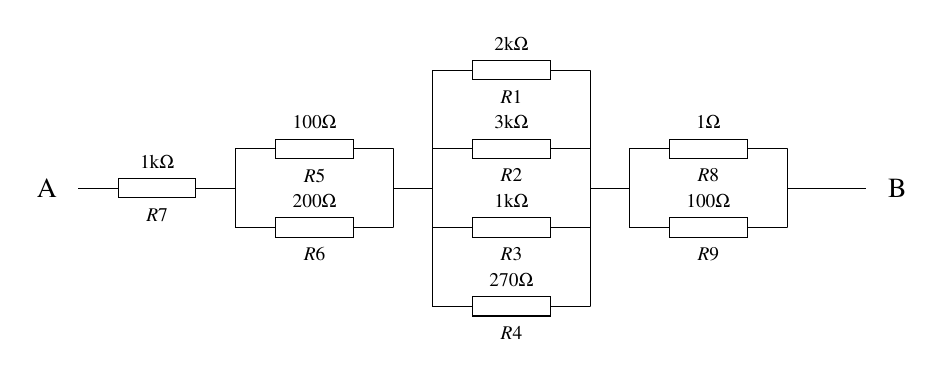
\begin{tikzpicture}[
    circuit ee IEC,
    x = 2cm, y = 1cm,
    every info/.style = {font = \scriptsize},
    set diode graphic = var diode IEC graphic,
    set make contact graphic = var make contact IEC graphic]

\draw (0,0) to [resistor={ohm=1k, info'={$R7$}}] (1,0) --
	  (1,0) to (1,0.5)--
	  (1,0.5) to [resistor={ohm=100, info'={$R5$}}] (2,0.5) --
	  (2,0.5) to (2,0)
	  (1,0) to (1,-0.5)--
	  (1,-0.5) to [resistor={ohm=200, info'={$R6$}}] (2,-0.5) --
	  (2,-0.5) to (2,0)--
	  (2,0) to (2.25,0)--
	  (2.25,0) to (2.25,1.5)--
	  (2.25,1.5) to [resistor={ohm=2k, info'={$R1$}}] (3.25,1.5) --
	  (3.25,1.5) to (3.25,0)
	  (2.25,0) to (2.25,-1.5)--
	  (2.25,-1.5) to [resistor={ohm=270, info'={$R4$}}] (3.25,-1.5) --
	  (3.25,-1.5) to (3.25,0)
	  (2.25,-0.5) to [resistor={ohm=1k, info'={$R3$}}] (3.25,-0.5)
	  (2.25,0.5) to [resistor={ohm=3k, info'={$R2$}}] (3.25,0.5)
	  (3.25,0) to (3.5,0) --
	  (3.5,0) to (3.5,0.5) --
	  (3.5, 0.5) to [resistor={ohm=1, info'={$R8$}}] (4.5, 0.5) --
	  (4.5, 0.5) to (4.5,0)
	  (3.5,0) to (3.5,-0.5) --
	  (3.5,-0.5) to [resistor={ohm=100, info'={$R9$}}] (4.5,-0.5) --
	  (4.5,-0.5) to (4.5,0) --
	  (4.5,0) to (5,0);  
\path (-0.2,0) node(x) {{A}}
	  (5.2,0) node(x) {{B}};
\end{tikzpicture}
\end{figure}



$$
R_{z} = R_{7} + \frac{R_{5}+R_{6}}{R_{5}\cdot R_{6}} + \frac{R_{1}\cdot R_{2}\cdot R_{3}+R_{1}\cdot R_{2}\cdot R_{4}+R_{1}\cdot R_{3}\cdot R_{4}+R_{2}\cdot R_{3}\cdot R_{4}}{R_{1}\cdot R_{2}\cdot R_{3}\cdot R_{4}} + \frac{R_{8}+R_{9}}{R_{8}\cdot R_{9}}
$$

\begin{center}
$R_{z} = 1k\Omega + \frac{100\Omega + 200\Omega}{100\Omega\cdot200\Omega} + \frac{1\Omega + 100\Omega}{1\Omega\cdot100\Omega}+$\\
\vspace{0,5cm}
\begin{large}
$+ \frac{2k\Omega\cdot3k\Omega\cdot1k\Omega + 2k\Omega\cdot3k\Omega\cdot270\Omega + 2k\Omega\cdot1k\Omega\cdot270\Omega + 3k\Omega\cdot1k\Omega\cdot270\Omega}{2k\Omega\cdot3k\Omega\cdot1k\Omega\cdot270\Omega}$\\
\end{large}
\end{center}
$$
R_{z} = 1000\Omega + 0,015\Omega + 1,01\Omega + 0,006\Omega = 1001,031\Omega
$$

\newpage
\subsection{Część 2.}
Obliczanie rezystancji obwodów oraz jej pomiar dla obwodu zbudowanego na płytce prototypowej.\\
Pod każdym przykładem zamieszczono porównanie obliczonej rezystancji z jej zmierzoną wartością.\\

\subsubsection{Obwód 1.}

\begin{figure}[!h]
\centering
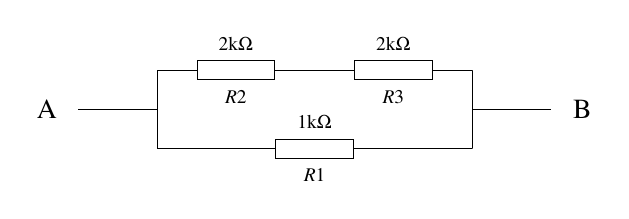
\begin{tikzpicture}[
    circuit ee IEC,
    x = 2cm, y = 1cm,
    every info/.style = {font = \scriptsize},
    set diode graphic = var diode IEC graphic,
    set make contact graphic = var make contact IEC graphic]

\draw (0,0) to (0.5,0) --
	  (0.5,0) to (0.5,0.5)--
	  (0.5,0.5) to [resistor={ohm=2k, info'={$R2$}}] (1.5,0.5) --
	  (1.5,0.5) to [resistor={ohm=2k, info'={$R3$}}] (2.5, 0.5) -- 
	  (2.5,0.5) to (2.5,0)
	  (0.5,0) to (0.5,-0.5)--
	  (0.5,-0.5) to [resistor={ohm=1k, info'={$R1$}}] (2.5,-0.5) --
	  (2.5,-0.5) to (2.5,0) --
	  (2.5,0) to (3,0); 
\path (-0.2,0) node(x) {{A}}
	  (3.2,0) node(x) {{B}};
\end{tikzpicture}
\end{figure}

$$
R_{z} = \frac{(R_{2}+R_{3})\cdot R_{1}}{R_{1}+R_{2}+R_{3}}
$$
\\
$$
R_{z} = \frac{(2k\Omega+2k\Omega)\cdot 1k\Omega}{1k\Omega+2k\Omega+3k\Omega}
$$
\\
\begin{tabular}{|c|c|}
\hline
\textbf{Obliczenia} & \textbf{Pomiar}\\
\hline
$800\Omega$ & $790\Omega$\\
\hline
\end{tabular}

\subsubsection{Obwód 2.}

\begin{figure}[!h]
\centering
\begin{tikzpicture}[
    circuit ee IEC,
    x = 2cm, y = 1cm,
    every info/.style = {font = \scriptsize},
    set diode graphic = var diode IEC graphic,
    set make contact graphic = var make contact IEC graphic]

\draw (0,0) to (0.5,0) --
	  (0.5,0) to (0.5,-0.5) --
	  (0.5,-0.5) to [resistor={ohm=100, info'={$R4$}}] (3.75,-0.5) --
	  (3.75,-0.5) to (3.75, 0)
	  (0.5,0) to (0.5,1) --
	  (0.5,1) to (0.75,1) --
	  (0.75,1) to (0.75,1.5) --
	  (0.75,1.5) to [resistor={ohm=1k, info'={$R1$}}] (1.75,1.5) --
	  (1.75,1.5) to (1.75,1)
	  (0.75,1) to (0.75,0.5) --
	  (0.75,0.5) to [resistor={ohm=2k, info'={$R2$}}] (1.75,0.5) --
	  (1.75,0.5) to (1.75,1) --
	  (1.75,1) to [resistor={ohm=1k, info'={$R3$}}] (2.75,1) --
	  (2.75,1) to [resistor={ohm=100, info'={$R5$}}] (3.75,1) --
	  (3.75,1) to (3.75,0)--
	  (3.75,0) to (4.25,0);
\path (-0.2,0) node(x) {{A}}
	  (4.45,0) node(x) {{B}};
\end{tikzpicture}
\end{figure}

$$
R_{z} = \frac{R_{4}\cdot(R_{1}\cdot R_{2} + (R_{1} + R_{2})\cdot(R_{3}+R_{5})}{R_{1}\cdot R_{2} + (R_{1}+R_{2})\cdot(R_{3}+R_{5}) + (R_{1}+R_{2})\cdot R_{4}}
$$
\\
$$
R_{z} = \frac{100\Omega\cdot(1k\Omega\cdot 2k\Omega + (1k\Omega + 2k\Omega)\cdot(1k\Omega+100\Omega)}{1k\Omega\cdot 2k\Omega + (1k\Omega+2k\Omega)\cdot(1k\Omega+100\Omega) + (1k\Omega+2k\Omega)\cdot 100\Omega}
$$
\\
\begin{tabular}{|c|c|}
\hline
\textbf{Obliczenia} & \textbf{Pomiar}\\
\hline
$94,6\Omega$ & $95\Omega$\\
\hline
\end{tabular}

\newpage
\subsubsection{Obwód 3.}

\begin{figure}[!h]
\centering
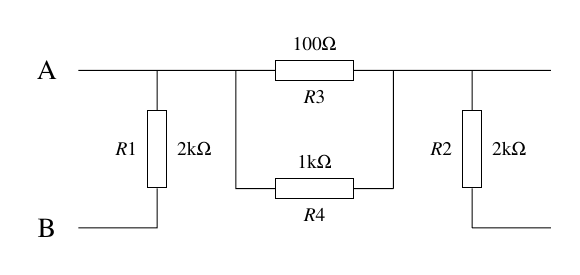
\begin{tikzpicture}[
    circuit ee IEC,
    x = 2cm, y = 1cm,
    every info/.style = {font = \scriptsize},
    set diode graphic = var diode IEC graphic,
    set make contact graphic = var make contact IEC graphic]

\draw (0,0) to (0.5,0) --
	  (0.5,0) to [resistor={ohm=2k, info'={$R1$}}] (0.5,-2) --
	  (0.5,-2) to (0, -2)
	  (0.5,0) to (1,0) --
	  (1,0) to [resistor={ohm=100, info'={$R3$}}] (2,0)
	  (1,0) to (1,-1.5) --
	  (1,-1.5) to [resistor={ohm=1k, info'={$R4$}}] (2,-1.5)--
	  (2,-1.5) to (2,0) --
	  (2,0) to (2.5,0) --
	  (2.5,0) to [resistor={ohm=2k, info'={$R2$}}] (2.5, -2) --
	  (2.5,-2) to (3,-2)
	  (2.5,0) to (3,0) ;
\path (-0.2,0) node(x) {{A}}
	  (-0.2,-2) node(x) {{B}};
\end{tikzpicture}
\end{figure}

$$
R_{z} = R_{1} = 2k\Omega
$$
\\
\begin{tabular}{|c|c|}
\hline
\textbf{Obliczenia} & \textbf{Pomiar}\\
\hline
$2k\Omega$ & $1,952k\Omega$\\
\hline
\end{tabular}

\subsubsection{Obwód 4.}

\begin{figure}[!h]
\centering
\begin{tikzpicture}[
    circuit ee IEC,
    x = 2cm, y = 1cm,
    every info/.style = {font = \scriptsize},
    set diode graphic = var diode IEC graphic,
    set make contact graphic = var make contact IEC graphic]

\draw (0,0) to (0.5,0) --
	  (0.5,0) to (0.5,-0.5) --
	  (0.5,-0.5) to [resistor={ohm=1k, info'={$R4$}}] (3.75,-0.5) --
	  (3.75,-0.5) to (3.75, 0)
	  (0.5,0) to (0.5,1) --
	  (0.5,1) to (0.75,1) --
	  (0.75,1) to (0.75,1.5) --
	  (0.75,1.5) to [resistor={ohm=100, info'={$R5$}}] (1.75,1.5) --
	  (1.75,1.5) to [resistor={ohm=1k, info'={$R1$}}] (2.75,1.5) --
	  (2.75,1.5) to (2.75,1)
	  (0.75,1) to (0.75,0.5) --
	  (0.75,0.5) to [resistor={ohm=2k, info'={$R2$}}] (2.75,0.5) --
	  (2.75,0.5) to (2.75,1)
	  (2.75,1) to [resistor={ohm=2k, info'={$R3$}}] (3.75,1) --
	  (3.75,1) to (3.75,0)--
	  (3.75,0) to (4.25,0);
\path (-0.2,0) node(x) {{A}}
	  (4.45,0) node(x) {{B}};
\end{tikzpicture}
\end{figure}

$$
R_{z} = \frac{R_{4}\cdot ((R_{1} + R_{5})\cdot R_{2} + (R_{1} + R_{2} + R_{5})\cdot R_{3})}{(R_{1} + R_{2} + R_{5})\cdot (R_{3} + R_{4}) + (R_{1} + R_{5})\cdot R_{2}}
$$
\\
$$
R_{z} = \frac{1k\Omega\cdot ((1k\Omega + 100\Omega)\cdot 2k\Omega + (1k\Omega + 2k\Omega + 100\Omega)\cdot 2k\Omega)}{(1k\Omega + 2k\Omega + 100\Omega)\cdot (2k\Omega + 1k\Omega) + (1k\Omega + 100\Omega)\cdot 2k\Omega}
$$
\\
\begin{tabular}{|c|c|}
\hline
\textbf{Obliczenia} & \textbf{Pomiar}\\
\hline
$730,4\Omega$ & $725\Omega$\\
\hline
\end{tabular}

\newpage
\subsubsection{Obwód 5.}

\begin{figure}[!h]
\centering
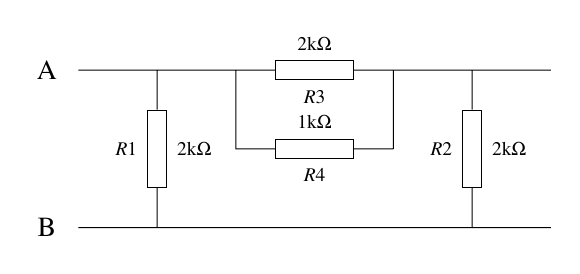
\begin{tikzpicture}[
    circuit ee IEC,
    x = 2cm, y = 1cm,
    every info/.style = {font = \scriptsize},
    set diode graphic = var diode IEC graphic,
    set make contact graphic = var make contact IEC graphic]

\draw (0,0) to (0.5,0) --
	  (0.5,0) to [resistor={ohm=2k, info'={$R1$}}] (0.5,-2) --
	  (0.5,-2) to (0, -2)
	  (0.5,0) to (1,0) --
	  (1,0) to [resistor={ohm=2k, info'={$R3$}}] (2,0)
	  (1,0) to (1,-1) --
	  (1,-1) to [resistor={ohm=1k, info'={$R4$}}] (2,-1)--
	  (2,-1) to (2,0) --
	  (2,0) to (2.5,0) --
	  (2.5,0) to [resistor={ohm=2k, info'={$R2$}}] (2.5, -2) --
	  (2.5,-2) to (3,-2)
	  (2.5,0) to (3,0) 
	  (0.5,-2) to (2.5,-2);
\path (-0.2,0) node(x) {{A}}
	  (-0.2,-2) node(x) {{B}};
\end{tikzpicture}
\end{figure}

$$
R_{z} = \frac{R_{1}\cdot(R_{3}\cdot R_{4} + R_{2}\cdot(R_{3} + R_{4}))}{R_{3}\cdot R_{4} + (R_{1}\cdot R_{2})\cdot (R_{3} + R_{4})}
$$ 
\\
$$
R_{z} = \frac{2k\Omega\cdot(2k\Omega\cdot 1k\Omega + 2k\Omega\cdot(2k\Omega + 1k\Omega))}{2k\Omega\cdot 1k\Omega + (2k\Omega\cdot 2k\Omega)\cdot (2k\Omega + 1k\Omega)}
$$ 
\\
\begin{tabular}{|c|c|}
\hline
\textbf{Obliczenia} & \textbf{Pomiar}\\
\hline
$1142,9\Omega$ & $1119\Omega$\\
\hline
\end{tabular}


\subsubsection{Obwód 6.}

\begin{figure}[!h]
\centering
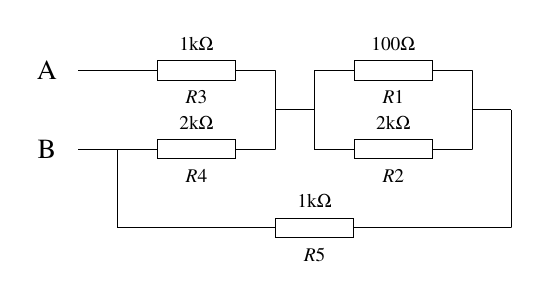
\begin{tikzpicture}[
    circuit ee IEC,
    x = 2cm, y = 1cm,
    every info/.style = {font = \scriptsize},
    set diode graphic = var diode IEC graphic,
    set make contact graphic = var make contact IEC graphic]

\draw (0,0) to (0.25,0) --
	  (0.25,0) to [resistor={ohm=1k, info'={$R3$}}] (1.25,0) --
	  (1.25,0) to (1.25, -0.5)
	  (0,-1) to (0.25,-1) --
	  (0.25,-1) to [resistor={ohm=2k, info'={$R4$}}] (1.25,-1)--
	  (1.25,-1) to (1.25,-0.5) --
	  (1.25,-0.5) to (1.5,-0.5) --
	  (1.5,-0.5) to (1.5,0) -- 
	  (1.5,0) to [resistor={ohm=100, info'={$R1$}}] (2.5,0)--
	  (2.5,0) to (2.5,-0.5)
	  (1.5,-0.5) to (1.5,-1) -- 
	  (1.5,-1) to [resistor={ohm=2k, info'={$R2$}}] (2.5,-1)--
	  (2.5,-1) to (2.5,-0.5)--
	  (2.5,-0.5) to (2.75, -0.5)
	  (0.25, -1) to (0.25, -2)--
	  (0.25, -2) to [resistor={ohm=1k, info'={$R5$}}] (2.75,-2)--
	  (2.75,-2) to (2.75,-0.5);
\path (-0.2,0) node(x) {{A}}
	  (-0.2,-1) node(x) {{B}};
\end{tikzpicture}
\end{figure}

W celu zwiększenia czytelności obliczeń, w tym przypadku wprowadzimy dodatkowe oznaczenia:
$$
R_{6} = \frac{R_{1}\cdot R_{2}}{R_{1}+R_{2}} = \frac{100\Omega\cdot 2k\Omega}{100\Omega+2k\Omega} = 95,24\Omega
$$
$$
R_{7} = R_{6} + R_{5} = 1000\Omega + 95,24\Omega = 1095,24\Omega
$$
$$
R_{8} = \frac{R_{4}\cdot R_{7}}{R_{4}+R_{7}} = \frac{2000\Omega\cdot 1095,24\Omega}{2000\Omega + 1095,24\Omega} = 707,7\Omega
$$
\\
$$
R_{z} = R_{3} + R_{8} = 1000\Omega + 707,7\Omega = 1707,7\Omega\\
$$
\\
\begin{tabular}{|c|c|}
\hline
\textbf{Obliczenia} & \textbf{Pomiar}\\
\hline
$1707,7\Omega$ & $1684\Omega$\\
\hline
\end{tabular}

\subsection{Podsumowanie}
W zadaniu widać było różnice pomiędzy obliczoną rezystancją i jej zmierzoną, rzeczywistą wartością. Różnice te mogą wynikać między innymi z 
:
\begin{itemize}
\item Niezerowego oporu przewodów płytki prototypowej i kabli użytych do podłączenia miernika;
\item Niepewności pomiarowych sprzętu użytego w doświadczeniu;
\item Ograniczonej precyzji wykonania opornika prowadzącej do różnicy między oporem nominalnym a rzeczywistym.
\end{itemize}



\section{Wnioski}
Zakładając poprawność przeprowadzonych badań jesteśmy w stanie stwierdzić, że dla częstotliwości równej... wg znanej nam wiedzy \cite{bolkowski1986teoria} zachodzi zjawisko rezonansu szeregowego, które pokrywa się z wartością obliczoną na podstawie wzorów algebraicznych \cite{bolkowski1986teoria}. Wszelkie rozbieżności mogą wynikać z...
\bibliographystyle{IEEEtran}

\bibliography{IEEEabrv,refs}

\end{document}

